\chapter{القلب والدورة القلبية}\label{ch:b2:heart}

اقطع \omterm{def:b2:heart:anatomy}{قلب} ضفدع وألقه في محلول ملحي، فيظل
ينبض ساعات --- بلا أعصاب، ولا دماغ، ولا دم، بل عضلة
تنقبض من تلقاء نفسها نحو مرة في الثانية لأن رقعة
صغيرة من خلاياها لا تستطيع السكون. \omterm{def:b2:heart:anatomy}{والقلب} البشري يفعل هذا
نحو ثلاثة مليارات مرة في العمر، فيحرك ما رتبته مئتا
مليون لتر، دون أن يُطفأ قط. وهذا
الفصل عن تلك المضخة: حجراتها ودسامتها، ودورة
الامتلاء والإفراغ والضغوط التي تقودها، والجملة الكهربائية
التي توقّتها والأثر الذي تتركه على الجلد، والقانون
الذي يتيح لها مطابقة نتاجها بوارِدها نبضةً بنبضة، و
الأعصاب والهرمونات التي تعدّل سرعتها وقوتها.

\section{المضخة}

\begin{definition}[الحجرات والدسامات]\label{def:b2:heart:anatomy}
\index{قلب}\index{أذين}\index{بطين}\index{دسام قلبي}
القلب مضختان جنبًا إلى جنب، لكل منهما \emph{أذين}
يتلقى الدم من الأوردة و\emph{بطين} يقذفه
إلى \omterm{def:b2:blood-circulation:vessels}{شريان}. فالقلب الأيمن يأخذ الدم من الأجوفين
ويرسله إلى الرئتين عبر \omterm{def:b2:blood-circulation:vessels}{الشريان} الرئوي؛ والقلب
الأيسر يستعيده من الأوردة الرئوية ويرسله حول
الجسم عبر الأبهر. وأربعة دسامات تجعل الجريان أحادي الاتجاه:
\emph{الدسامان الأذينيان البطينيان} (المثلث الشرف على اليمين، والتاجي
على اليسار)، وهما وريقات مربوطة بحبال إلى عضلات حليمية بحيث
لا يمكن دفعها راجعةً إلى الأذين؛ و
\emph{الدسامان الهلاليان} (الرئوي والأبهري)، وهما ثلاثة جيوب
تمتلئ وتُحكم الإغلاق حين يفوق الضغط الشرياني ضغط البطين.
والدسامات سلبية: فهي تنفتح وتنغلق على فروق الضغط
وحدها. وجدار البطين \emph{عضلة قلبية}، وهي
عضل مخطط من خلايا متفرعة موصولة طرفًا إلى طرف
\emph{بأقراص بينية} مملوءة بالوصلات الفجوية، فيكون البطين
كله خلية واحدة كهربائيًا وينقبض وحدةً واحدة؛ وجدار
البطين الأيسر أثخن ثلاث مرات من الأيمن لأنه
يضخ ضد خمسة أضعاف الضغط. وتغذي عضلةَ القلب
شرايينُها \emph{الإكليلية}، التي تمتلئ في الانبساط، وهي
تعمل باستقلاب هوائي كله تقريبًا --- فلا تستطيع الاستدانة.
\end{definition}

\begin{omfigure}
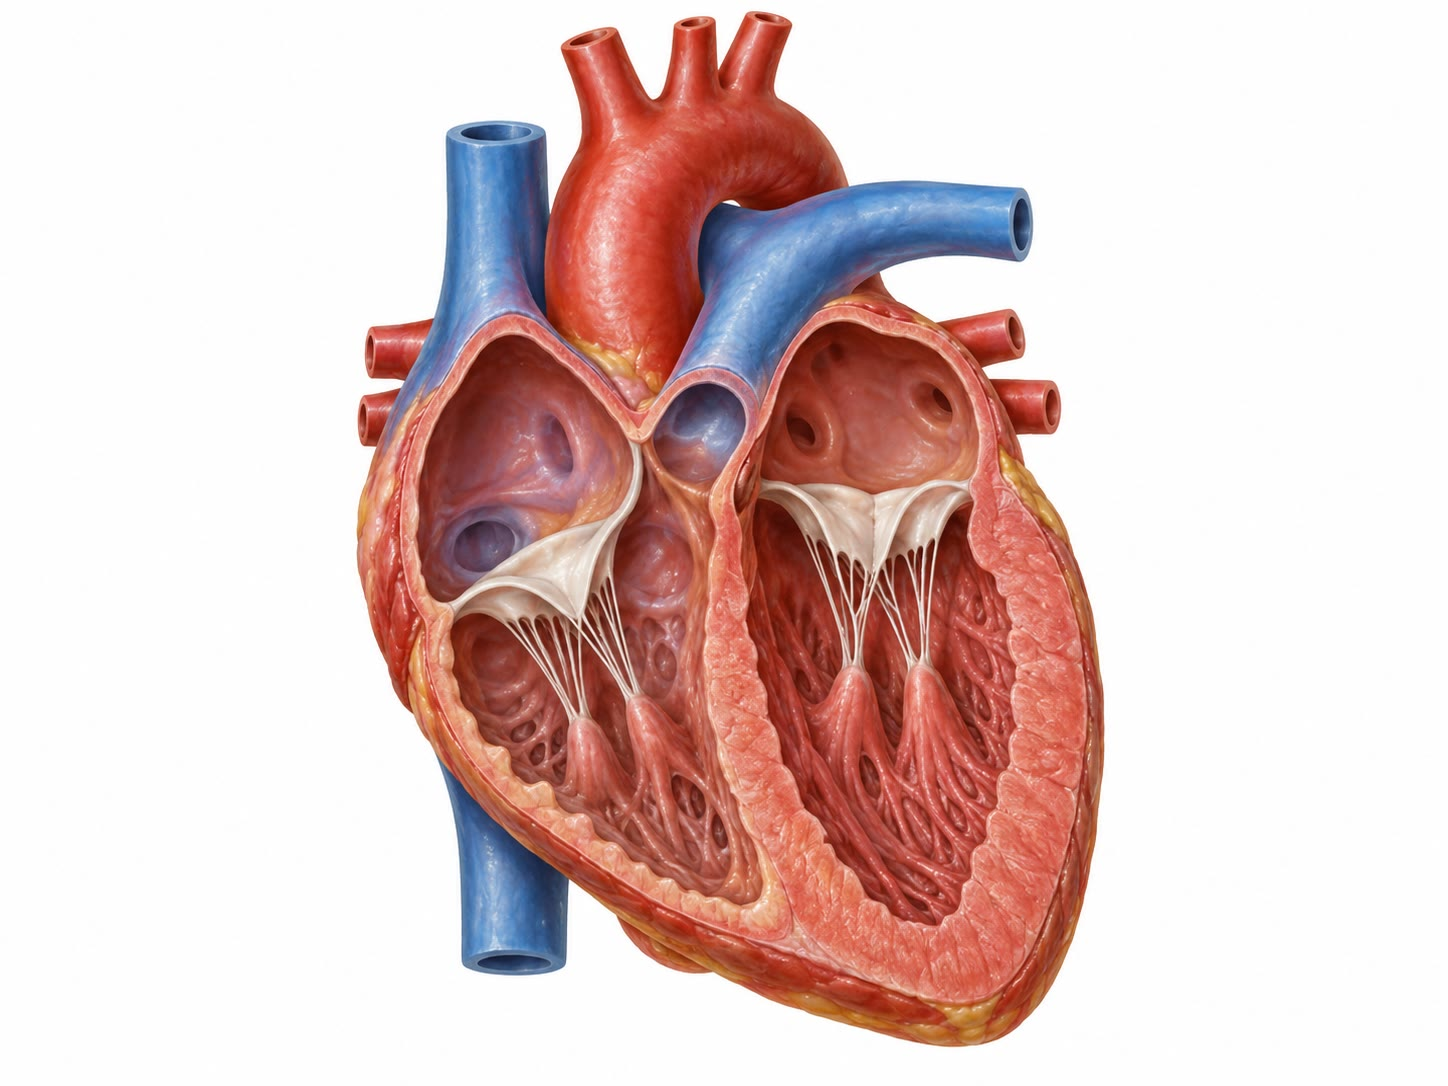
\includegraphics[width=0.55\linewidth]{images/book4/ai/b4-17-heart-cutaway.jpg}

{\small \omterm{def:b2:heart:anatomy}{القلب} في مقطع أمامي: أذينان في الأعلى، وبطينان
في الأسفل، \omterm{def:b2:heart:anatomy}{والبطين} الأيسر السميك، والدسامان الأذينيان البطينيان بحبالهما،
والشريانان الكبيران يغادران من الأعلى.}
\end{omfigure}

\begin{proposition}[الدورة القلبية]\label{prop:b2:heart:cycle}
\index{دورة قلبية}\index{انقباض}\index{انبساط}\index{حجم الضربة}\index{كسر القذف}
تدوم نبضة واحدة في الراحة نحو \qty{0.8}{s}. و\emph{الانبساط}
(\qty{0.5}{s}): ترتخي البطينان، ويهبط ضغطهما دون ضغط
الأذينين، فينفتح الدسامان الأذينيان البطينيان ويجري الدم داخلًا،
سلبيًا في معظمه، ثم بدفعة أخيرة من انقباض الأذينين؛
وينهي \omterm{def:b2:heart:anatomy}{البطين} الانبساط حاملًا نحو \qty{120}{mL} (وهو
\emph{الحجم نهاية الانبساط}). و\emph{الانقباض} (\qty{0.3}{s}):
ينقبض البطينان؛ وما إن يفوق ضغطهما ضغط
الأذينين حتى ينغلق الدسامان الأذينيان البطينيان (وهو الصوت القلبي الأول،
«لُبّ»)، ويعصر \omterm{def:b2:heart:anatomy}{البطين} حجرةً مغلقة بضعة أجزاء من مئة من الثانية
--- أي \emph{الانقباض متساوي الحجم} ---
حتى يتجاوز ضغطه الضغط الشرياني (\qty{80}{mmHg} على
اليسار)، فينفتح الدسامان الهلاليان ويُقذف الدم. و
يبلغ \omterm{def:b2:heart:anatomy}{البطين} الأيسر \qty{120}{mmHg} ويدفع نحو
\qty{70}{mL} (وهو \emph{\omterm{prop:b2:heart:cycle}{حجم الضربة}}، أي \emph{كسر قذف}
قدره \qty{60}{\%})؛ وإذ يرتخي يهبط ضغطه دون ضغط
الأبهر، فيُطبق الدسام الأبهري (وهو الصوت الثاني، «دُبّ»)،
ويهبط ارتخاء متساوي الحجم بالضغط إلى مستوى
\omterm{def:b2:heart:anatomy}{الأذين}، فيستأنف الامتلاء. \omterm{def:b2:heart:anatomy}{والقلب} الأيمن يفعل الشيء نفسه
بخمس الضغط، ويقذف الحجم نفسه.
\end{proposition}

\begin{omfigure}
\begin{tikzpicture}
\begin{axis}[
  width=0.9\linewidth, height=7.2cm,
  axis x line=bottom, axis y line=left,
  xmin=0, xmax=0.8, ymin=0, ymax=130,
  xlabel={الزمن في الدورة (ث)}, ylabel={الضغط (\unit{mmHg})},
  xlabel style={font=\small, at={(axis description cs:0.5,-0.1)}, anchor=north},
  ylabel style={font=\small},
  tick label style={font=\small}, xtick={0,0.1,0.3,0.8}, ytick={0,40,80,120},
  legend style={font=\scriptsize, at={(0.6,0.45)}, anchor=west, draw=none},
  clip=false,
]
% aortic pressure
\addplot[very thick, omThm] coordinates {(0,82) (0.05,80) (0.1,80) (0.12,95) (0.16,115) (0.2,120) (0.25,112) (0.3,100) (0.32,104) (0.34,100) (0.45,94) (0.6,88) (0.8,82)};
\addlegendentry{الأبهر}
% left ventricular pressure
\addplot[very thick, omDef] coordinates {(0,5) (0.04,8) (0.05,10) (0.08,60) (0.1,80) (0.12,95) (0.16,115) (0.2,120) (0.25,112) (0.3,100) (0.32,60) (0.35,20) (0.38,5) (0.5,3) (0.7,5) (0.75,8) (0.8,5)};
\addlegendentry{البطين الأيسر}
% atrial pressure
\addplot[thick, omProp] coordinates {(0,6) (0.03,9) (0.06,6) (0.1,8) (0.15,6) (0.3,7) (0.36,10) (0.4,5) (0.6,6) (0.75,9) (0.8,6)};
\addlegendentry{الأذين الأيسر}
\draw[dashed, gray] (axis cs:0.05,0) -- (axis cs:0.05,128); \node[font=\scriptsize, anchor=south, align=center] at (axis cs:0.05,128) {التاجي\\ينغلق};
\draw[dashed, gray] (axis cs:0.1,0) -- (axis cs:0.1,128); \node[font=\scriptsize, anchor=south, align=center] at (axis cs:0.13,128) {الأبهري\\ينفتح};
\draw[dashed, gray] (axis cs:0.31,0) -- (axis cs:0.31,128); \node[font=\scriptsize, anchor=south, align=center] at (axis cs:0.31,128) {الأبهري\\ينغلق};
\draw[dashed, gray] (axis cs:0.38,0) -- (axis cs:0.38,128); \node[font=\scriptsize, anchor=south, align=center] at (axis cs:0.4,128) {التاجي\\ينفتح};
\node[font=\scriptsize] at (axis cs:0.2,45) {انقباض};
\node[font=\scriptsize] at (axis cs:0.55,25) {انبساط};
\end{axis}
\end{tikzpicture}

{\small الضغوط في \omterm{def:b2:heart:anatomy}{القلب} الأيسر خلال نبضة واحدة. يعصر \omterm{def:b2:heart:anatomy}{البطين}
حجرةً مغلقة حتى يتجاوز الضغط الأبهري، ثم
يقذف ما دام فوقه، ثم يرتخي حتى يهبط دون ضغط
\omterm{def:b2:heart:anatomy}{الأذين}، ثم يمتلئ.}
\end{omfigure}

\begin{theorem}[شغل القلب]\label{thm:b2:heart:work}
\index{شغل قلبي}\index{حلقة الضغط--الحجم}
مرسومةً ضغطًا بدلالة الحجم، ترسم نبضة واحدة من \omterm{def:b2:heart:anatomy}{البطين} الأيسر
حلقةً --- امتلاءً على طول الأسفل، وانقباضًا متساوي
الحجم صعودًا على اليمين، وقذفًا على طول الأعلى من
\qty{120}{mL} إلى \qty{50}{mL}، وارتخاءً متساوي الحجم نزولًا على
اليسار --- ومساحة الحلقة هي الشغل الميكانيكي
للنبضة:
\[
W = \oint P\,\mathrm{d}V \approx \bar P_{\text{القذف}}\times \text{حجم الضربة} \approx \qty{100}{mmHg}\times\qty{70}{mL} = \qty{0.93}{J}.
\]
وعند 72 نبضة في الدقيقة يبذل \omterm{def:b2:heart:anatomy}{البطين} الأيسر نحو \qty{1.1}{W}، والأيمن
\qty{0.2}{W}؛ واستقلاب \omterm{def:b2:heart:anatomy}{القلب} نحو \qty{8}{W}، فيكون مردوده
الميكانيكي قريبًا من \qty{15}{\%}، والباقي حرارة و
كلفة التوتر. ورفع الضغط الذي يضخ \omterm{def:b2:heart:anatomy}{القلب} ضده
(فرط التوتر، أو دسام أبهري متضيق) يرفع الشغل في النبضة
بالتناسب، وتثخن العضلة استجابةً كما تفعل كل عضلة
--- حتى لا تعود تروية شرايينها الإكليلية تجاري ضخامتها.
\end{theorem}
\begin{proof}
الشغل قوة في مسافة، ومن أجل ضغط يعمل على جدار
متحرك، فهو ضغط في حجم مكنوس: أي $\mathrm{d}W = P\,\mathrm{d}V$.
وعلى حلقة مغلقة يكون الشغل الصافي المساحةَ المحاطة (فالامتلاء عند
ضغط منخفض يكلف قليلًا؛ والقذف عند ضغط عالٍ يعيد أكثر
بكثير). و$\qty{100}{mmHg} = \qty{1.33e4}{Pa}$ و$\qty{70}{mL} =
\qty{7e-5}{m^3}$: ومنه $1.33\times 10^{4}\times 7\times 10^{-5} =
\qty{0.93}{J}$؛ وفي $1.2$ نبضة في الثانية، \qty{1.1}{W}.
\end{proof}

\begin{omfigure}
\begin{tikzpicture}
\begin{axis}[
  width=0.62\linewidth, height=6cm,
  axis x line=bottom, axis y line=left,
  xmin=0, xmax=150, ymin=0, ymax=140,
  xlabel={حجم البطين الأيسر (\unit{mL})}, ylabel={الضغط (\unit{mmHg})},
  xlabel style={font=\small, at={(axis description cs:0.5,-0.12)}, anchor=north},
  ylabel style={font=\small},
  tick label style={font=\small}, xtick={0,50,120}, ytick={0,80,120},
  clip=false,
]
\fill[omDef!12] (axis cs:50,5) -- (axis cs:120,8) -- (axis cs:120,80) -- (axis cs:110,115) -- (axis cs:80,122) -- (axis cs:50,100) -- cycle;
\draw[very thick, omDef, ->] (axis cs:50,5) -- (axis cs:120,8);
\draw[very thick, omDef, ->] (axis cs:120,8) -- (axis cs:120,80);
\draw[very thick, omDef, ->] (axis cs:120,80) .. controls (axis cs:110,118) and (axis cs:80,125) .. (axis cs:50,100);
\draw[very thick, omDef, ->] (axis cs:50,100) -- (axis cs:50,5);
\node[font=\scriptsize, anchor=south] at (axis cs:85,11) {امتلاء};
\node[font=\scriptsize, anchor=west] at (axis cs:122,44) {انقباض متساوي الحجم};
\node[font=\scriptsize, anchor=south] at (axis cs:85,124) {قذف};
\node[font=\scriptsize, anchor=east] at (axis cs:48,52) {ارتخاء};
\node[font=\scriptsize] at (axis cs:85,60) {المساحة $=$ الشغل، \qty{0.9}{J}};
\end{axis}
\end{tikzpicture}

{\small \omterm{thm:b2:heart:work}{حلقة الضغط--الحجم} \omterm{def:b2:heart:anatomy}{للبطين} الأيسر. والمساحة
المحاطة شغل نبضة واحدة؛ والضغط الشرياني الأعلى يرفع
أعلى الحلقة ويرفع الشغل معه.}
\end{omfigure}

\section{ساعة القلب الخاصة}

\begin{proposition}[الآلية الذاتية والتوصيل]\label{prop:b2:heart:conduction}
\index{العقدة الجيبية الأذينية}\index{ناظم الخطى}\index{العقدة الأذينية البطينية}\index{ألياف بركنجي}
تنشأ النبضة في \emph{\omterm{prop:b2:heart:conduction}{العقدة الجيبية الأذينية}}، وهي رقعة من
خلايا عضلية متخصصة في جدار \omterm{def:b2:heart:anatomy}{الأذين} الأيمن لا يستريح
كمون غشائها أبدًا: فبعد كل كمون فعل ينجرف
صاعدًا ببطء (وهو \emph{كمون \omterm{prop:b2:heart:conduction}{ناظم الخطى}}، يقوده
تيار صوديوم يشتغل عند الكمونات السالبة وتقوده قنوات
الكالسيوم) حتى يبلغ العتبة فينطلق من جديد، نحو
مئة مرة في الدقيقة لو تُرك وشأنه. وتنتشر الدفعة عبر
عضل الأذينين، خلية إلى خلية عبر الوصلات الفجوية، فينقبض
الأذينان؛ وتبلغ \emph{\omterm{prop:b2:heart:conduction}{العقدة الأذينية البطينية}}، وهي
الجسر الكهربائي الوحيد بين الأذينين والبطينين، وهي توصّل
ببطء وتؤخرها عُشر ثانية --- وهو زمن يكفي للأذينين
لإتمام ملء البطينين؛ ثم تنطلق نازلةً في
\emph{حزمة هيس} و\emph{\omterm{prop:b2:heart:conduction}{ألياف بركنجي}}، وهي خلايا سريعة التوصيل
تسلّمها إلى عضل البطينين كله في غضون
\qty{30}{ms}، فينقبض البطينان من الذروة صاعدًا،
وحدةً واحدة، ويدفعان الدم نحو دسامي الخروج. وكل
جزء من هذه الجملة يستطيع أن ينظّم بنفسه، وكل واحد أبطأ من
الذي قبله (فالعقدة عند 100، \omterm{prop:b2:heart:conduction}{والعقدة الأذينية البطينية} عند 50، \omterm{prop:b2:heart:conduction}{وألياف بركنجي} عند
30)، فإذا أخفقت العقدة تولّى مركز أدنى --- بمعدل
أبطأ.
\end{proposition}
\begin{proof}[شواهد]
\omterm{def:b2:heart:anatomy}{القلب} المعزول، أو شريحة من نسيج جيبي أذيني، ينبض في طبق
بلا أعصاب؛ وتنبض شريحة من \omterm{def:b2:heart:anatomy}{البطين} أيضًا، لكن أبطأ.
وتبريد \omterm{prop:b2:heart:conduction}{العقدة الجيبية الأذينية} وحدها أو تدفئتها يغير معدل
\omterm{def:b2:heart:anatomy}{القلب} كله؛ وقطع الحزمة الأذينية البطينية يفصل البطينين،
فينبضان عندئذ بإيقاعهما البطيء بينما يواصل الأذينان
بإيقاع العقدة (وهو الحصار القلبي). والتسجيل من خلية عقدة واحدة
يُظهر استقطاب الانبساط البطيء الذي لا تملكه أي خلية
عضلية عادية؛ وسدّ تيار \omterm{prop:b2:heart:conduction}{ناظم الخطى} يبطئه.
\end{proof}

\begin{omfigure}
\begin{tikzpicture}[every node/.style={font=\scriptsize}, >=stealth]
  % simplified heart outline, scaled up
  \draw[thick, fill=omThm!6] (0,0) .. controls (-4.2,1.3) and (-3.8,5.4) .. (-1.3,5.8) .. controls (0,6.1) and (0.6,5.6) .. (1.3,5.8) .. controls (3.8,5.4) and (4.2,1.3) .. (0,0);
  \draw[thick] (-3.0,3.5) .. controls (-0.8,3.85) and (0.8,3.85) .. (3.0,3.5);
  \draw[thick] (0,3.75) -- (0,0.6);
  \node at (-1.5,4.7) {الأذين الأيمن}; \node at (1.5,4.7) {الأذين الأيسر};
  \node[align=center] at (-1.3,2.55) {البطين\\الأيمن}; \node[align=center] at (1.3,2.55) {البطين\\الأيسر};
  % SA node
  \fill[omDef] (-2.5,5.0) circle (0.16); \node[omDef, anchor=east] at (-3.3,5.4) {العقدة الجيبية}; \draw[omDef] (-3.3,5.35) -- (-2.62,5.08);
  \draw[omDef, dashed] (-2.5,5.0) circle (0.45); \draw[omDef, dashed] (-2.5,5.0) circle (0.8);
  % AV node
  \fill[omDef] (-0.25,3.7) circle (0.14); \node[omDef, anchor=west] at (0.15,4.05) {العقدة الأذينية البطينية}; \draw[omDef] (0.15,4.05) -- (-0.12,3.78);
  % bundle and Purkinje
  \draw[very thick, omDef] (-0.25,3.6) -- (-0.25,2.1);
  \draw[very thick, omDef] (-0.25,2.1) .. controls (-0.8,1.4) .. (-1.9,1.1);
  \draw[very thick, omDef] (-0.25,2.1) .. controls (0.8,1.4) .. (1.9,1.1);
  \foreach \p in {(-1.9,1.1),(1.9,1.1)} { \draw[omDef] \p -- ++(-0.3,0.6); \draw[omDef] \p -- ++(0.3,0.7); \draw[omDef] \p -- ++(0,0.85); }
  \node[omDef, anchor=west] at (3.4,1.0) {ألياف بركنجي}; \draw[omDef] (3.4,1.0) -- (2.2,1.1);
  \node[omDef, anchor=east] at (-0.45,3.05) {حزمة هيس};
  % timing
  \node[anchor=west, align=left] at (5.6,5.0) {العقدة الجيبية تنطلق: $t = 0$\\الأذينان يستقطبان: 0--\qty{80}{ms}};
  \node[anchor=west, align=left] at (5.6,3.5) {تأخر العقدة الأذينية البطينية: \qty{100}{ms}};
  \node[anchor=west, align=left] at (5.6,1.9) {الحزمة وألياف بركنجي:\\البطينان مستقطبان\\بحلول \qty{220}{ms}، والذروة أولًا};
\end{tikzpicture}

{\small جملة التوصيل. تنطلق \omterm{prop:b2:heart:conduction}{العقدة الجيبية الأذينية}، فيستقطب الأذينان،
وتؤخر \omterm{prop:b2:heart:conduction}{العقدة الأذينية البطينية} الدفعة، وتسلّمها
الحزمة \omterm{prop:b2:heart:conduction}{وألياف بركنجي} إلى البطينين من الذروة صاعدًا.}
\end{omfigure}

\begin{proposition}[تخطيط القلب الكهربائي]\label{prop:b2:heart:ecg}
\index{تخطيط القلب الكهربائي}
\omterm{def:b2:heart:anatomy}{القلب} كتلة كبيرة من الخلايا تستقطب وتعيد الاستقطاب
بالتعاقب، والتيارات التي تجري في الجسم حوله يمكن
تسجيلها فولطياتٍ من مليفولط بين أقطاب على
الأطراف: وهو \emph{\omterm{prop:b2:heart:ecg}{تخطيط القلب الكهربائي}}. وموجاته أحداث
جملة التوصيل: \emph{فالموجة P} استقطاب الأذينين؛
و\emph{الفترة PR} المستوية (\qty{0.16}{s}) هي تأخر \omterm{prop:b2:heart:conduction}{العقدة الأذينية البطينية}؛
و\emph{المركّب QRS}، وهو حاد قصير (\qty{0.08}{s})، استقطاب
البطينين --- وهو كبير لأن كتلة البطينين كبيرة، وقصير
لأن \omterm{prop:b2:heart:conduction}{ألياف بركنجي} سريعة؛ و\emph{الموجة T} إعادة استقطاب
البطينين. (أما إعادة استقطاب الأذينين فمدفونة في
QRS.) والأثر يبلّغ عن التوقيت والتوصيل، لا عن القوة: \omterm{prop:b2:heart:conduction}{فالعقدة
الأذينية البطينية} المحصورة تطيل الفترة PR أو تفصل P عن QRS، والمنطقة الميتة
من \omterm{def:b2:heart:anatomy}{البطين} تشوّه QRS، \omterm{def:b2:heart:anatomy}{والأذين} غير المنتظم (الرجفان
الأذيني) يستبدل بالموجات P ضجيجًا ويجعل البطينين
ينبضان بلا انتظام، والفترة بين موجتي R تعطي المعدل.
\end{proposition}

\begin{omfigure}
\begin{tikzpicture}
\begin{axis}[
  width=0.9\linewidth, height=5.2cm,
  axis x line=bottom, axis y line=left,
  xmin=0, xmax=1.0, ymin=-0.4, ymax=1.3,
  xlabel={الزمن (ث)}, ylabel={مليفولط},
  xlabel style={font=\small, at={(axis description cs:0.5,-0.12)}, anchor=north},
  ylabel style={font=\small},
  tick label style={font=\small}, xtick={0,0.2,0.4,0.6,0.8,1.0}, ytick={0,1},
  clip=false,
]
\addplot[very thick, omDef] coordinates {(0,0) (0.08,0) (0.1,0.05) (0.14,0.15) (0.18,0.05) (0.2,0) (0.28,0) (0.3,-0.1) (0.31,0) (0.33,1.1) (0.35,0) (0.36,-0.25) (0.375,0) (0.5,0) (0.54,0.1) (0.58,0.28) (0.62,0.1) (0.65,0) (0.88,0) (0.9,0.05) (0.94,0.15) (0.98,0.05) (1.0,0)};
\node[font=\scriptsize, anchor=south] at (axis cs:0.14,0.17) {P};
\node[font=\scriptsize, anchor=south] at (axis cs:0.33,1.12) {R};
\node[font=\scriptsize, anchor=north] at (axis cs:0.295,-0.11) {Q};
\node[font=\scriptsize, anchor=north] at (axis cs:0.365,-0.27) {S};
\node[font=\scriptsize, anchor=south] at (axis cs:0.58,0.3) {T};
\draw[<->, gray] (axis cs:0.1,0.45) -- (axis cs:0.3,0.45); \node[font=\scriptsize, anchor=south, gray] at (axis cs:0.2,0.46) {PR \qty{0.16}{s}};
\draw[<->, gray] (axis cs:0.3,0.6) -- (axis cs:0.375,0.6); \node[font=\scriptsize, anchor=west, gray] at (axis cs:0.38,0.6) {QRS \qty{0.08}{s}};
\draw[<->, gray] (axis cs:0.33,1.25) -- (axis cs:0.94,1.25); \node[font=\scriptsize, anchor=south, gray] at (axis cs:0.63,1.25) {الفترة R--R $=$ 60/المعدل};
\end{axis}
\end{tikzpicture}

{\small تخطيط \omterm{def:b2:heart:anatomy}{قلب} كهربائي سوي: P (الأذينان)، وتأخر PR عند
\omterm{prop:b2:heart:conduction}{العقدة الأذينية البطينية}، وQRS (استقطاب البطينين)، وT (إعادة استقطاب
البطينين).}
\end{omfigure}

\section{تنظيم النتاج}

\begin{theorem}[قانون فرانك--ستارلنغ]\label{thm:b2:heart:starling}
\index{قانون فرانك--ستارلنغ}\index{الحمل القبلي}\index{نتاج قلبي}
ترتفع قوة انقباض \omterm{def:b2:heart:anatomy}{البطين} مع الحجم الذي
ملأه: ففي مجال العمل، كلما تمدد \omterm{def:b2:heart:anatomy}{البطين} أكثر
في الانبساط (وهو \emph{\omterm{thm:b2:heart:starling}{الحمل القبلي}})، قذف أكثر في
الانقباض. \omterm{def:b2:heart:anatomy}{فالقلب} إذن يضخ خارجًا، نبضةً بنبضة، كل ما
يتلقاه --- فارتفاع العود الوريدي \qty{20}{\%} يقابله ارتفاع
في \omterm{prop:b2:heart:cycle}{حجم الضربة} قدره \qty{20}{\%} بلا أي عصب أو هرمون --- و
البطينان، اللذان يجب أن يحركا الحجم نفسه، يوازن أحدهما
الآخر تلقائيًا: فإذا سلّم \omterm{def:b2:heart:anatomy}{القلب} الأيمن دمًا أكثر إلى
الرئتين، تلقى \omterm{def:b2:heart:anatomy}{القلب} الأيسر أكثر وضخ أكثر. والآلية
في \omterm{def:b2:cell-differentiation:fibre}{القسيم العضلي}: فعند الأطوال القصيرة \omterm{def:b2:heart:anatomy}{لبطين} سيئ
الامتلاء يفرط تداخل الخيوط الغليظة والرفيعة وتكون
حساسية الكالسيوم منخفضة؛ والتمدد نحو الطول الأمثل
(\qty{2.2}{\micro m}) يزيد التداخل المتاح
للجسور المستعرضة والحساسيةَ معًا، فتنتج نبضة الكالسيوم نفسها
قوة أكبر. وفوق الأمثل (أي \omterm{def:b2:heart:anatomy}{قلب} مفرط التمدد
عاطل) تهبط القوة من جديد.
\end{theorem}
\begin{proof}[شواهد]
سجّل فرانك (1895) الضغط الذي يولّده \omterm{def:b2:heart:anatomy}{بطين} ضفدع
مملوء إلى أحجام مختلفة: فارتفع ضغط الذروة مع حجم
الامتلاء حتى حد أقصى ثم هبط. وبيّن ستارلنغ (1914)، في
تحضير قلب--رئة كلب يمكن فيه ضبط العود الوريدي والمقاومة
الشريانية على حدة، أن رفع العود يرفع النتاج ضربةً
بضربة، وأن رفع المقاومة الشريانية يقابله، بعد بضع نبضات من التراكم،
حجمٌ أكبر عند نهاية الانبساط ونتاجٌ مستعاد --- \omterm{def:b2:heart:anatomy}{فالبطين}
يجيب الحمل بالتمدد ويجيب التمدد بانقباض أشد.
\end{proof}

\begin{omfigure}
\begin{tikzpicture}
\begin{axis}[
  width=0.66\linewidth, height=5.4cm,
  axis x line=bottom, axis y line=left,
  xmin=0, xmax=200, ymin=0, ymax=140,
  xlabel={الحجم عند نهاية الانبساط (\unit{mL})}, ylabel={حجم الضربة (\unit{mL})},
  xlabel style={font=\small, at={(axis description cs:0.5,-0.13)}, anchor=north},
  ylabel style={font=\small},
  tick label style={font=\small}, xtick={0,50,100,150,200}, ytick={0,50,100},
  legend style={font=\scriptsize, at={(0.5,-0.3)}, anchor=north, draw=none, legend columns=3},
  clip=false,
]
\addplot[very thick, omDef, domain=40:200, samples=60] {130*(1-exp(-(x-40)/70))};
\addlegendentry{سوي}
\addplot[very thick, omThm, domain=40:200, samples=60] {130*1.3*(1-exp(-(x-40)/55))};
\addlegendentry{مع تنبيه ودّي}
\addplot[very thick, omExo!70!black, domain=40:200, samples=60] {130*0.5*(1-exp(-(x-40)/90))};
\addlegendentry{قلب عاطل}
\fill[omDef] (axis cs:120,88) circle (2pt); \node[font=\scriptsize, anchor=south east] at (axis cs:118,90) {راحة};
\end{axis}
\end{tikzpicture}

{\small منحنيات ستارلنغ. يرتفع \omterm{prop:b2:heart:cycle}{حجم الضربة} مع الامتلاء؛ و
الأعصاب الودّية تزيح المنحني صاعدًا (فنتاج أكبر من الامتلاء
نفسه)، \omterm{def:b2:heart:anatomy}{والقلب} العاطل يزيحه نازلًا.}
\end{omfigure}

\begin{proposition}[الأعصاب والهرمونات]\label{prop:b2:heart:control}
\index{الجملة العصبية الودّية!القلب}\index{العصب المبهم}\index{الأدرينالين}\index{نتاج قلبي}
\omterm{thm:b2:heart:starling}{النتاج القلبي} هو معدل \omterm{def:b2:heart:anatomy}{القلب} في \omterm{prop:b2:heart:cycle}{حجم الضربة}، أي \qty{5}{L/min}
في الراحة وحتى \qty{25}{L/min} في جهد رياضي مدرَّب.
وكلا العاملين تضبطه الأعصاب الذاتية. أما \emph{المبهم}
(نظير الودّي) فهو، بإطلاقه الأستيل كولين على \omterm{prop:b2:heart:conduction}{العقدة الجيبية الأذينية}،
يبطئ انجراف \omterm{prop:b2:heart:conduction}{ناظم الخطى} ويبقي معدل الراحة عند 70 بدل
مئة العقدة نفسها؛ واقطع المبهمين يرتفع المعدل. أما
الأعصاب \emph{الودّية}، بإطلاقها النورأدرينالين، ولب الكظر،
بإطلاقه \emph{الأدرينالين} في الدم، فتسرّع الانجراف
(فنبضات أكثر)، وتسرّع التوصيل، وترفع قوة الانقباض
عند أي امتلاء (أي منحني ستارلنغ أشد ميلًا، وهي الخاصة المسماة
\emph{القابلية للانقباض})، برفعها الكالسيوم المسلَّم إلى
القسيمات العضلية في كل نبضة. وفي الجهد يُرفع كابح المبهم
أولًا، ثم يُضغط مسرّع الودّي، فيعطي معدل 180
مع حجم ضربة \qty{140}{mL} مقدار \qty{25}{L/min}؛ و
تُرحَّل الإشارات عبر مستقبلات ورسل ثوانٍ في
\cref{ch:b2:cell-signalling}، ويقود الكلَّ مراكز
تنظيم الضغط في \cref{ch:b2:blood-pressure}.
\end{proposition}

\begin{example}[قراءة قلب]\label{ex:b2:heart:reading}
صوتان في النبضة: «لُبّ»، وهو انغلاق الدسامين الأذينيين البطينيين في مطلع
الانقباض؛ و«دُبّ»، وهو انغلاق الدسامين الهلاليين في نهايته. واللغط
جريان مضطرب عبر دسام متضيق (وهو تضيق) أو راجع
عبر دسام راشح (وهو قصور): فاللغط بين «لُبّ» و
«دُبّ» دسام تاجي راشح أو دسام أبهري متضيق، وبعد «دُبّ»
دسام أبهري راشح. ونبض قدره 70 مع ضغط دم
$120/80$~ملم زئبق يعني حجم ضربة قريبًا من \qty{70}{mL}؛
ومعدل 40 عند رياضي يعني حجم ضربة كبيرًا وتوترًا
مبهميًا قويًا؛ ومعدل 40 مع فترة PR تطول حتى تسقط
نبضة يعني عقدة أذينية بطينية مريضة. وفيزيولوجيا هذا الفصل هي
ما يسمعه الطبيب بسماعته في ثلاثين ثانية.
\end{example}

\section{تمارين}

\begin{exercise}[$\star$]\label{exo:b2:heart:1}
تتبّع قطرة دم من الأجوف إلى الأبهر، مسمّيًا كل
حجرة ودسام ووعاء بالترتيب.
\end{exercise}

\begin{exercise}[$\star$]\label{exo:b2:heart:2}
أعط أطوار \omterm{prop:b2:heart:cycle}{الدورة القلبية} مع حالة كل دسام
في كل طور، والحدث الذي يسبب كلًا من الصوتين
القلبيين.
\end{exercise}

\begin{exercise}[$\star$]\label{exo:b2:heart:3}
سمِّ أجزاء جملة التوصيل بالترتيب، مع الزمن الذي تستغرقه
الدفعة لتبلغ كل جزء، والموجة التي ينتجها كل جزء في التخطيط.
\end{exercise}

\begin{exercise}[$\star$]\label{exo:b2:heart:4}
اذكر \omterm{thm:b2:heart:starling}{قانون فرانك--ستارلنغ} وقل لماذا يضمن أن يضخ
البطينان الحجم نفسه.
\end{exercise}

\begin{exercise}[$\star\star$]\label{exo:b2:heart:5}
\omterm{def:b2:heart:anatomy}{قلب} حجمه عند نهاية الانبساط \qty{130}{mL} وحجمه عند
نهاية الانقباض \qty{50}{mL} عند 70 نبضة في الدقيقة. احسب
\omterm{prop:b2:heart:cycle}{حجم الضربة} \omterm{prop:b2:heart:cycle}{وكسر القذف} \omterm{thm:b2:heart:starling}{والنتاج القلبي}. \omterm{def:b2:heart:anatomy}{وقلب}
عاطل حجماه \qty{180}{mL} و\qty{120}{mL}: أعد الحساب، وقل
ماذا حدث \omterm{prop:b2:heart:cycle}{لكسر القذف}.
\end{exercise}

\begin{exercise}[$\star\star$]\label{exo:b2:heart:6}
احسب شغل نبضة من أجل حجم ضربة \qty{70}{mL} عند
ضغط قذف متوسط \qty{100}{mmHg}، والاستطاعة عند 72 نبضة
في الدقيقة. وأعد الحساب من أجل مصاب بفرط التوتر عند \qty{150}{mmHg}. وكم
أكسجينًا زائدًا في الدقيقة يحتاج \omterm{def:b2:heart:anatomy}{القلب} الثاني، إذا كان
المردود الميكانيكي \qty{15}{\%} وكان \qty{1}{mL} من الأكسجين
يعطي \qty{20}{J}؟
\end{exercise}

\begin{exercise}[$\star\star$]\label{exo:b2:heart:7}
في تخطيط \omterm{def:b2:heart:anatomy}{قلب} تبعد موجتا R \qty{0.5}{s} في تسجيل و
\qty{1.5}{s} في آخر. أعط معدلي \omterm{def:b2:heart:anatomy}{القلب}. وفي ثالث، تأتي الموجات P
كل \qty{0.6}{s} والمركّبات QRS كل \qty{1.8}{s}، بلا
علاقة ثابتة. فماذا حدث؟
\end{exercise}

\begin{exercise}[$\star\star$]\label{exo:b2:heart:8}
ينجرف كمون خلية \omterm{prop:b2:heart:conduction}{العقدة الجيبية الأذينية} من \qty{-60}{mV} إلى
عتبة \qty{-40}{mV} بمعدل \qty{25}{mV/s} قبل كل كمون
فعل مدته \qty{0.15}{s}. احسب الفترة بين النبضات و
المعدل. والأستيل كولين يخفض الانجراف إلى \qty{18}{mV/s} و
كمون البداية إلى \qty{-65}{mV}؛ والنورأدرينالين يرفع الانجراف
إلى \qty{40}{mV/s}. احسب المعدلين.
\end{exercise}

\begin{exercise}[$\star\star$]\label{exo:b2:heart:9}
اشرح لماذا يكون تأخر \omterm{prop:b2:heart:conduction}{العقدة الأذينية البطينية} لازمًا، وماذا كان ليحدث
للنتاج بدونه، ولماذا تكون العقدة البطيئة (أي الفترة PR الطويلة)
غير ضارة إلى حد ثم خطرة بعده.
\end{exercise}

\begin{exercise}[$\star\star\star$]\label{exo:b2:heart:10}
رياضي في الراحة معدله 45 ونتاجه \qty{5}{L/min}؛
وفي الجهد معدله 180 ونتاجه \qty{30}{L/min}. احسب حجمي
الضربة وقل بماذا يسهم منحني ستارلنغ والأعصاب الودّية
في كل منهما. ولماذا لا يستطيع المعدل أن يتجاوز نحو 200 بفائدة؟
\end{exercise}

\begin{exercise}[$\star\star\star$]\label{exo:b2:heart:11}
دسام أبهري متضيق يترك فتحة \qty{1}{cm^2} بدل
\qty{3}{cm^2}. باستعمال الاستمرارية، احسب سرعة الدم
المقذوف عند \qty{250}{mL/s} عبر كل منهما، واحسب، من برنولي
($\Delta P = \tfrac12\rho v^2$)، الضغط الذي على \omterm{def:b2:heart:anatomy}{البطين} أن
يولّده فوق الضغط الأبهري في كل حالة. وماذا يفعل
\omterm{def:b2:heart:anatomy}{البطين} حيال ذلك، وما الكلفة في النهاية؟
\end{exercise}

\begin{exercise}[$\star\star\star$]\label{exo:b2:heart:12}
«\omterm{def:b2:heart:anatomy}{القلب} مضخة تنظّم نفسها ولا تعدّلها إلا
الجملة العصبية.» ناقش، مميّزًا ما توفره الآلية الذاتية و
\omterm{thm:b2:heart:starling}{قانون فرانك--ستارلنغ} والأعصاب الذاتية، وما الذي
يستطيعه وما لا يستطيعه \omterm{def:b2:heart:anatomy}{قلب} مزروع --- وهو بلا أعصاب.
\end{exercise}

\section{مسألة: قلب تحت حمل}

\begin{problem}[{مسألة نهاية الأسبوع --- متابعة قلب واحد من الراحة إلى
الجهد وإلى المرض: توقيت دورته، وحساب شغله، وقراءة
تخطيطه الكهربائي، وقياس استجابته الستارلنغية وتحكمه الذاتي،
وتقدير كلفة دسام متضيق، وتنتهي إلى
النتاج في الراحة وفي الجهد، والشغل في النبضة، و
التدرج عبر التضيق}]
\label{pb:b2:heart:1}
المعطيات: في الراحة، المعدل 70، والحجم عند نهاية الانبساط \qty{130}{mL}،
وعند نهاية الانقباض \qty{60}{mL}، وضغط القذف المتوسط \qty{100}{mmHg}
($\qty{1}{mmHg} = \qty{133}{Pa}$)، والضغط الأبهري $120/80$~ملم زئبق.
ويدوم الانقباض \qty{0.3}{s} عند أي معدل. \omterm{prop:b2:heart:conduction}{وناظم الخطى}: انجراف من
\qty{-60}{mV} إلى \qty{-40}{mV}، وكمون الفعل \qty{0.15}{s}. و
يستهلك \omterm{def:b2:heart:anatomy}{القلب} \qty{20}{J} لكل مليلتر أكسجين بمردود
ميكانيكي قدره \qty{15}{\%}؛ ويحمل الدم الإكليلي
\qty{0.2}{mL} من الأكسجين في المليلتر ويستخلص \omterm{def:b2:heart:anatomy}{القلب}
\qty{70}{\%} منه. وكثافة الدم \qty{1060}{kg/m^3}.

\medskip
\noindent\textbf{الجزء الأول --- الدورة في الراحة.}
\begin{enumerate}
  \item احسب \omterm{prop:b2:heart:cycle}{حجم الضربة} \omterm{prop:b2:heart:cycle}{وكسر القذف} \omterm{thm:b2:heart:starling}{والنتاج
        القلبي}.
  \item احسب مدة دورة واحدة ومدة الانبساط.
  \item احسب معدل القذف المتوسط خلال الانقباض،
        بالمليلترات في الثانية، والسرعة المتوسطة عبر
        دسام أبهري \qty{3}{cm^2}.
  \item يرتفع ضغط \omterm{def:b2:heart:anatomy}{البطين} بمعدل \qty{1500}{mmHg/s} خلال
        الانقباض متساوي الحجم، من 10 إلى \qty{80}{mmHg}. فكم
        يدوم ذلك الطور؟
  \item احسب شغل نبضة واحدة والاستطاعة الميكانيكية
        \omterm{def:b2:heart:anatomy}{للبطين} الأيسر.
  \item احسب استطاعة \omterm{def:b2:heart:anatomy}{القلب} الكلية واستهلاكه من الأكسجين
        (البطينين معًا: خذ الأيمن خمس الأيسر).
  \item احسب الجريان الدموي الإكليلي اللازم لتوفير ذلك الأكسجين.
\end{enumerate}

\medskip
\noindent\textbf{الجزء الثاني --- \omterm{prop:b2:heart:conduction}{ناظم الخطى} والأثر.}
\begin{enumerate}[resume]
  \item أي معدل انجراف (\unit{mV/s}) يعطي معدلًا قدره 70؟
  \item يُقطع المبهم: فيصير المعدل 100. فأي معدل انجراف
        هذا؟
  \item احسب معدل الانجراف من أجل معدل 180 في الجهد.
  \item في تخطيط الراحة، أعط الفترة R--R، وقل ماذا تقابل
        الموجات P وQRS وT.
  \item الفترة PR \qty{0.16}{s} في الراحة. وطولها في معظمه
        تأخر \omterm{prop:b2:heart:conduction}{العقدة الأذينية البطينية}: اشرح ما يحققه التأخر
        ولماذا يقتضي معدل 180 أن تسرّع العقدة هي أيضًا.
  \item يُظهر تخطيط مريض مركّبات QRS كل \qty{1.5}{s} وموجات P
        كل \qty{0.8}{s}، بلا علاقة. شخّص، وأعط
        المعدل البطيني، وقل أي نسيج ينظّم
        البطينين.
\end{enumerate}

\medskip
\noindent\textbf{الجزء الثالث --- الجهد.}
في الجهد يرتفع المعدل إلى 180 وترفع الأعصاب الودّية
القابلية للانقباض فيهبط الحجم عند نهاية الانقباض إلى
\qty{30}{mL}؛ ويرفع العود الوريدي الحجم عند نهاية الانبساط إلى
\qty{150}{mL}.
\begin{enumerate}[resume]
  \item احسب \omterm{prop:b2:heart:cycle}{حجم الضربة} \omterm{prop:b2:heart:cycle}{وكسر القذف} والنتاج.
  \item احسب مدة الانبساط عند 180 واشرح لماذا لا يستطيع
        المعدل أن يعلو كثيرًا بفائدة.
  \item احسب استطاعة \omterm{def:b2:heart:anatomy}{البطين} الأيسر عند ضغط قذف
        متوسط \qty{120}{mmHg}، واستهلاك \omterm{def:b2:heart:anatomy}{القلب} من
        الأكسجين.
  \item احسب الجريان الإكليلي اللازم، وقارنه بالراحة.
        ولماذا يكون قصر الانبساط مشكلة له؟
  \item دون الأعصاب الودّية (أي \omterm{def:b2:heart:anatomy}{قلب} مزروع) لا يرتفع
        المعدل إلا ببطء، عبر الأدرينالين في الدم، وترتفع
        القابلية للانقباض أقل. تنبّأ بالنتاج في الدقيقة الأولى
        من الجهد، مستعملًا قانون ستارلنغ وحده بالامتلاء نفسه.
  \item انسب ارتفاع النتاج من الراحة إلى الجهد إلى
        أسبابه الثلاثة (المعدل، والامتلاء، والقابلية للانقباض)، باللترات في
        الدقيقة لكل سبب.
\end{enumerate}

\medskip
\noindent\textbf{الجزء الرابع --- دسام متضيق.}
يتضيق الدسام الأبهري إلى \qty{1}{cm^2}.
\begin{enumerate}[resume]
  \item احسب سرعة القذف في الراحة عبر الدسام
        المتضيق.
  \item باستعمال برنولي، $\Delta P = \tfrac12\rho v^{2}$، احسب
        الضغط الذي على \omterm{def:b2:heart:anatomy}{البطين} أن يضيفه ليدفع الدم عبره،
        بملم الزئبق.
  \item أعد حساب الاثنين في الجهد.
  \item ماذا يجب أن يكون ضغط ذروة \omterm{def:b2:heart:anatomy}{البطين} في كل حالة
        لإبقاء الضغط الأبهري سويًا، وبأي عامل يرتفع
        شغله في النبضة في الراحة؟
  \item يثخن جدار \omterm{def:b2:heart:anatomy}{البطين} استجابةً. اشرح لماذا يساعد ذلك
        ولماذا يخفق في النهاية (فكّر في التروية
        الإكليلية وفي الامتلاء الانبساطي).
  \item اذكر النتيجة: النتاج في الراحة وفي الجهد، و
        الشغل في النبضة في الراحة، والتدرج عبر الدسام
        المتضيق في الراحة وفي الجهد.
\end{enumerate}
\end{problem}
